\documentclass[landscape]{article}
\usepackage[a4paper,margin=3mm,landscape]{geometry}
\usepackage[scaled=0.92]{helvet}
\usepackage{multicol, multirow}
\usepackage{makecell}
\usepackage{array} 
\usepackage[table]{xcolor}
\usepackage{enumitem} 
\usepackage{amssymb}
\usepackage{graphicx}
\setlist{nosep}

\graphicspath{{./images/}}

\pdfinfo{
    /Title (ACC1701X Cheatsheet.pdf)
    /Creator (TeX)
    /Producer (pdfTeX 1.40.0)
    /Author (Andre Chua and Selwyn Ang)
    /Subject (ACC1701X)
    /Keywords (ACC1701X, Cheatsheet, NUS, Accounting) 
}

% Turn off header and footer
\pagestyle{empty}


\makeatletter
\DeclareRobustCommand\smaller{\@setfontsize\smaller{6pt}{6.5pt}}
\makeatother

% redefine section commands to use less space
\makeatletter
\renewcommand{\section}{\@startsection{section}{1}{0mm}%
  {-0.1ex plus -0.1ex minus -0.1ex}%
  {0.1ex plus .1ex minus 0.1ex}%
{\normalfont\small\bfseries}}
\renewcommand{\subsection}{\@startsection{subsection}{2}{0mm}%
  {-0.1ex plus -0.1ex minus -0.1ex}%
  {0.1ex plus .1ex minus 0.1ex}%
{\normalfont\scriptsize\bfseries}}
\renewcommand{\subsubsection}{\@startsection{subsubsection}{3}{0mm}%
  {-0.1ex plus -0.1ex minus -0.1ex}%
  {0.1ex plus .1ex minus 0.1ex}%
{\normalfont\smaller\bfseries}}%
\makeatother



\renewcommand{\familydefault}{\sfdefault}
\renewcommand\rmdefault{\sfdefault}
%  makes nested numbering (e.g. 1.1.1, 1.1.2, etc)
\renewcommand{\labelenumii}{\theenumii}
\renewcommand{\theenumii}{\theenumi.\arabic{enumii}.}
\renewcommand\labelitemii{•}
\renewcommand\labelitemiii{•}

\setlength{\parindent}{0pt}
\setlength{\parskip}{0pt plus 0.5ex}
\setlength{\columnsep}{0.2cm}
%% adjust spacing for all itemize/enumerate
\setlength{\leftmargini}{0.5cm}
\setlength{\leftmarginii}{0.5cm}
\setlist[itemize,1]{leftmargin=2mm,labelindent=1mm,labelsep=1mm}
\setlist[itemize,2]{leftmargin=2mm,labelindent=1mm,labelsep=1mm}
\setlist[itemize,3]{leftmargin=2mm,labelindent=1mm,labelsep=1mm}
\setlist[enumerate,1]{leftmargin=2mm,labelindent=1mm,labelsep=1mm}
\setlist[enumerate,2]{leftmargin=2mm,labelindent=1mm,labelsep=1mm}
\setlist[enumerate,3]{leftmargin=2mm,labelindent=1mm,labelsep=1mm}

% tightcenter
\newenvironment{tightcenter}{%
  \setlength\topsep{0pt}
  \setlength\parskip{0pt}
  \begin{center}
    }{%
  \end{center}
}

% boxed
\newenvironment{tightbox}{%
  \setlength\topsep{0pt}
  \setlength\parskip{0pt}
  \begin{center}
    \begin{tabular}{|@{\hspace{\dimexpr\fboxsep+0.5\arrayrulewidth}}c@{\hspace{\dimexpr\fboxsep+0.5\arrayrulewidth}}|}
      \hline
    }
    {%
    \\ \hline
    \end{tabular}
  \end{center}
}

% fixed width box
\newenvironment{fixedbox}[1][0.7]{
  \setlength\topsep{0pt}
  \setlength\parskip{0pt}
  \begin{center}
    \begin{tabular}{|>{\centering\arraybackslash}m{#1\linewidth}|}
    \hline
  }{
  \\ \hline
  \end{tabular}
  \end{center}
}

% definition of a new term
\usepackage{soul}
\definecolor{paleyellow}{RGB}{251,243,218}
\newcommand{\definition}[2][]{\sethlcolor{paleyellow}\hl{\textbf{#2}} #1  $\rightarrow$}
% inline definition
\newcommand{\ildefinition}[1]{\sethlcolor{paleyellow}\hl{\textbf{#1}}}

% important note (attention)
\newcommand{\attention}{{\color{red}\textbf{! }}}

% nice proof
\newenvironment{niceproof}[1][Proof]
{%
  \sbox0{\textit{#1}. }%
  \list{}{\labelwidth\wd0 \leftmargin\wd0 \labelsep 0pt }
\item[\usebox0]}
  {\endlist}


\usepackage{color, soul}
\usepackage{listings}
\usepackage{inconsolata}

\definecolor{codegreen}{rgb}{0,0.6,0}
\definecolor{codegray}{rgb}{0.5,0.5,0.5}
\definecolor{codepurple}{HTML}{C42043}
\definecolor{backcolour}{HTML}{F2F2F2}
\definecolor{bookColor}{cmyk}{0,0,0,0.90}

\newcommand{\code}[1]{\texttt{\sethlcolor{backcolour}\hl{$\,$#1$\,$}}}

% SQL code blocks
% define SQL styles
\lstdefinestyle{mySQL}{%
  language=SQL,
  backgroundcolor=\color{backcolour},
  commentstyle=\color{codegreen},
  keywordstyle=\color{codepurple},
  numberstyle=\numberstyle,
  stringstyle=\color{codepurple},
  basicstyle=\scriptsize\ttfamily,
  breaklines=true,
}



% --------------------------------------------------------

\begin{document}
\raggedright
\tiny
\begin{multicols}{6}
    \setlength{\columnseprule}{0.25pt}

    \begin{tightcenter}
        \fbox{%
          \parbox{0.8\linewidth}{\centering \textcolor{black}{
              {\Large\textbf{ACC1701X}}
            \\ \normalsize{AY23/24 SEM 2}}
            \\ {\footnotesize \textcolor{gray}{github/andrechuakj}}
            \\ {\footnotesize \textcolor{gray}{github/SelwynAng}}
          }%
        }
    \end{tightcenter}
    
    \section{Overview of Financial Statements}

    \subsection{Balance Sheet}

      \begin{itemize}
        \item \textbf{Assets:} Cash, AR, Inventory, Buildings
        \item \textbf{Liabilities:} AP, Income Tax Payable, Mortgage Payable, Unearned Revenue
        \item \textbf{Equity:} Capital Stock, Retained Earnings
      \end{itemize}

      \begin{fixedbox}[0.9]
        Assets = Liabilities + Equity
      \end{fixedbox}

      \begin{itemize}
        \item \textbf{Current Assets:} Cash \& other assets that are expected to be converted to cash or consumed within a year
        \item \textbf{Current Liabilities:} Obligations expected to be satisfied within a year.
      \end{itemize}

      \textbf{Limitations of Balance Sheet}
      \begin{itemize}
        \item Assets are recorded at purchase cost, not current market value
        \item Not all economic assets are included
        \item Accouting book value (equity) is usually $<$ market value (Market price per share * No. of shares)
      \end{itemize}
    
    \subsection{Statement of Comprehensive Income}
      \begin{itemize}
        \item \textbf{Revenue}
        \item \textbf{Expenses:} Operating (e.g. utilities, salary, rental, depreciation) \& Non-Operating (e.g. interest, income tax)
        \item \textbf{Net income}
        \item \textbf{Other comprehensive income}
      \end{itemize}

      \begin{fixedbox}[0.9]
        (1) \textbf{Net Income} = Revenue - Expenses
        \\ (2) \textbf{CI} = Net Income + Other CI
        \\(3) \textbf{Gross Profit} = Sales - COGS
        \\(4) \textbf{Earnings per share} = Net Income / No. of outstanding shares
      \end{fixedbox}

    \subsection{Statement of Change in Equity}
      \begin{fixedbox}[0.9]
        \textbf{Equity$_{ending}$} = Equity$_{beginning}$ + $\Uparrow$ Capital Stock + Net Income - Dividends + Other CI
      \end{fixedbox}
      
      \begin{itemize}
        \item \textbf{Retained Earnings:} Amount of business' net income retained in business
      \end{itemize}
      \begin{fixedbox}[0.9]
        \textbf{Retained Earnings$_{ending}$}
        \\= RE$_{beginning}$ + Net Income - Dividends
      \end{fixedbox}

    \subsection{Statement of Cash Flows}
      \begin{fixedbox}[0.9]
        \textbf{Cash Balance$_{ending}$} = Cash Balance$_{beginning}$ + Operating Activities + Investing Activities + Financing Activities
      \end{fixedbox}

    \subsection{Notes to the Financial Statements}
      \begin{itemize}
        \item Summary of Significant Accounting Policies
        \item Additional Info about Summary Totals
        \item Disclosure of Info not recognised in Financial Statements
        \item Supplementary Info required under Accounting Standards
      \end{itemize}
    \subsection{Concepts and Assumptions}
      \begin{itemize}
        \item \textbf{Separate Entity Concept:} Activities of a business entity are separated from those of the individual owners
        \item \textbf{Time-period Assumption:} Idea used to report the results of activities over a standard time period, which usually monthly, quarterly or annually
        \item \textbf{Assumption of Arm's length Transactions:} Business dealings between independent and rational parties who are looking out for their own interests
        \item \textbf{Cost Principle:} Idea that transactions are recorded at their historical costs / exchange prices at the transaction date
        \item \textbf{Fair Value Principle:} Idea that assets and liabilities should be measured at fair value to increase relevance of accounting information
        \item \textbf{Monetary Measurement Concept:} Value of item must be measurable in dollar value \& only economic activities measurable in monetary terms are included in the accounting model
        \item \textbf{Going Concern Assumption:} Idea that an accounting entity will have a continuing existence for the foreseeable future
      \end{itemize}

    \section{Mechanics of Accounting}
    
    \subsection{Anaylyse Transactions}
    
    Only the following exchange transactions will be recorded:
    \begin{itemize}
      \item Involve exchange of resources
      \item Conducted at arm's length between 2 entities
      \item Can be reliably measured in monetary terms
    \end{itemize}
    \textbf{Counter example:} Signing of employment contract (Have not started work yet) / giving offer to sell  G\&S (No actual sales) are not exchange transactions

    \subsection{Record Transactions}
    \textbf{Types of T-accounts}
    \begin{itemize}
      \item \textbf{Assets:}
        \begin{itemize}
          \item \textit{Current Assets:} Cash, Notes receivable, AR, Inventory, Supplies
          \item \textit{Non-current Assets:} Land, Buildings, Office Equipment
        \end{itemize}
      \item \textbf{Liabilities:}
        \begin{itemize}
          \item \textit{Current Liabilities:} Notes Payable, AP, Salaries Payable, Interest Payable, Income Taxes Payable
          \item \textit{Non-current Liabilities:} Mortgage Payable
        \end{itemize}
        \item \textbf{Equity:} Capital stock, Retained Earnings
        \item \textbf{Revenues:} Sales Revenue, Service Revenue
        \item \textbf{Expenses:} COGS, Salaries expenses, Interest expenses, Income Tax expense
    \end{itemize}

    \textbf{Debit \& Credit for T-accounts}
    \begin{itemize}
      \item \textbf{DR(+), CR(-):} Assets, Expenses, Dividends
      \item \textbf{DR(-), CR(+):} Liabilities, Equity, Capital Stock, Retained Earnings, Revenues
    \end{itemize}

    \textbf{Journal Entries to take note}
    \begin{itemize}
      \item \textbf{Selling goods:} \underline{DR Cash, CR Sales Revenue, DR COGS, CR Inventory}
      \item \textbf{Paying obligations \& Interest:} \underline{DR Notes Payable, DR Interest Expense, CR Cash}
      \item \textbf{Acquire cash from shareholders:} \underline{DR Cash, CR Capital Stock}
    \end{itemize}

    \subsection{Summarise Transactions}
    \begin{itemize}
      \item Journal Entries are posted to T-accounts
      \item Asset/Expense/Dividend normally have DR Balance
      \item Liability/Equity/Revenue normally have CR Balance
      \item Trial Balance is created from ending balances of all T-accounts (DR side == CR side)
    \end{itemize}

    \section{Accrual Accounting}

    \subsection{Accrual VS Cash-basis Accounting}
    \begin{itemize}
      \item \textbf{Accrual:} Revenue is recognised even if cash is not received; Expenses can be recorded even if cash is not paid
      \item \textbf{Cash:} Revenue \& expenses are recognised only when cash is received or paid
    \end{itemize}

    \subsection{Adjusting Entries}
    \subsubsection{Unrecorded Receivables (Asset)}
    \begin{itemize}
      \item Revenue earned during a period that have not been recorded by the end of that period
      \item Represent Asset to be collected in the future
      \item \textbf{Adjusting Entry:} \underline{DR AR, CR Revenue}
      \item E.g. Gave service to customer, but have not received cash
    \end{itemize}
    \subsubsection{Unrecorded Liabilities (Liability)}
    \begin{itemize}
      \item Expenses incurred \& not paid during a period and are not recorded at end of period
      \item Represent Liability to be paid in the future
      \item \textbf{Adjusting Entry:} \underline{DR Expense, CR AP}
      \item E.g. Received service from worker but have not paid worker OR Unrecorded interest payable
    \end{itemize}

    \subsubsection{Prepaid Expenses (Asset)}
    \begin{itemize}
      \item Payments made in advance for expense items
      \item \textbf{Journal Entry:} \underline{DR Prepaid Expense, CR Cash} OR \\ \hspace{1.1cm} \underline{DR Supplies, CR Cash}
      \item \textbf{Adjusting Entry:} \underline{DR Expense, CR Prepaid Expense} OR \\ \hspace{1.28cm} \underline{DR Supplies Expense, CR Supplies}
    \end{itemize}
    \subsubsection{Unearned Revenue (Liability)}
    \begin{itemize}
      \item Cash amounts received from customers before its corresponding revenue can be recognised
      \item \textbf{Journal Entry:} \underline{DR Cash, CR Unearned Revenue}
      \item \textbf{Adjusting Entry:} \underline{DR Unearned Revenue, CR Revenue}
    \end{itemize}

    \subsubsection{Summary of Adjusting Entries}
      \begin{tabular}{|l|l|l|}
      \hline
       &
        \textbf{\begin{tabular}[c]{@{}l@{}}Company give \\ service\end{tabular}} &
        \textbf{\begin{tabular}[c]{@{}l@{}}Company receive \\ service\end{tabular}} \\ \hline
      \textbf{\begin{tabular}[c]{@{}l@{}}Paid in \\ advance\end{tabular}} &
        \begin{tabular}[c]{@{}l@{}}Unearned \\ Revenue\end{tabular} &
        \begin{tabular}[c]{@{}l@{}}Prepaid \\ Expense\end{tabular} \\ \hline
      \textbf{\begin{tabular}[c]{@{}l@{}}Pay \\ later\end{tabular}} &
        \begin{tabular}[c]{@{}l@{}}Unrecorded \\ Receivables\end{tabular} &
        \begin{tabular}[c]{@{}l@{}}Unrecorded \\ Liabilities\end{tabular} \\ \hline
      \end{tabular}
      \underline{NOTE:} Each AE involves BS, SCI accts ONLY
    \subsection{Preparing Reports}
    \begin{enumerate}
      \item Prepare Unadjusted Trial Balance
      \item Prepare AEs
      \item Post AEs to T-accounts
      \item Prepare Adjusted Trial Balance (DR side = CR side)
      \item Prepare SCI based on Adjusted Trial Balance
      \item Compute Ending Retained Earnings balance
      \item Prepare Balance Sheet from Adjusted Trial Balance \& Ending Retained Earnings balance
      \item Prepare Statement of Cash Flows
      \item Prepare Notes to Financial Statements
      \item Close books (Post closing JEs to transfer all revenue, expense, dividend accounts balance to Retained Earnings account)
    \end{enumerate}

    \section{Revenue \& Receivables}

    \subsection{Revenue Recognition}
    \begin{enumerate}
      \item Identify contract with customer
      \item Identify performance obligations in contract
      \item Determine transaction price
      \item Allocate transaction price to separate performance obligations
      \item Determine when performance obligations are satisfied \& revenue can be recognised
    \end{enumerate}
    \subsection{AR, Cash, Revenue}
    \begin{itemize}
      \item \textbf{Credit Sales made:} \underline{DR AR, CR Sales Revenue}
      \item \textbf{Cash collected from Credit Sales:} \underline{DR Cash, CR AR}
      \item \textbf{Cash Sales made and cash collected:} \underline{DR Cash, CR Sales Revenue}
    \end{itemize}

    \subsection{Sales Discount and Sales Return and Allowances}
    \subsubsection{Sales Discount}
    \begin{itemize}
      \item Encourages early payment
      \item Sales Discount Account accumulates amount of sales discounts for all customers
      \item Credit terms: 2/10, n/30 (2\% discount if cash paid within 10 days, otherwise full amount due in 30 days)
      \item \textbf{Journal Entry:} \underline{DR Cash, DR Sales Discount, CR AR}
    \end{itemize}
    \subsubsection{Sales Returns \& Allowances}
    \begin{itemize}
      \item Customers have a right to return unsatisfactory/damaged merchandise \& receive a refund
      \item \textbf{Journal Entry:} \underline{DR Cash, DR Sales R\&A, CR AR} (Record cash collection \& sales return), \underline{DR Inventory, CR COGS} (Record cost of inventory returned)
    \end{itemize}
    \subsubsection{Net Sales}
    \begin{itemize}
      \item Sales Discount and Sales Return \& Allowances are contra-revenue accounts $\rightarrow$ Deducted from gross sales to derive net sales
    \end{itemize}
    \begin{fixedbox}
      Sales Revenue \hrulefill XXX
      \\ Less: Sales Discount \hrulefill (XXX)
      \\ Less: Sales R\&A \hrulefill (XXX)
      \\ Net Sales \hrulefill XXX
    \end{fixedbox}

    \subsection{Treatment of Bad Debts}
    \textit{\textbf{Bad Debts:}} Uncollectible AR
    \\\textit{\textbf{Expected Credit Loss:}} Estimated expense for uncollectible amount of AR (operating expense in SCI)
    \\\textit{\textbf{Loss Allowance:}} Contra-AR account on balance sheet, impairment of AR that is estimated to be uncollectible for all customers
    \subsubsection{Allowed Treatment of Bad Debts}
    \begin{itemize}
      \item \textbf{Journal Entry:} \underline{DR Expected Credit Loss, CR Loss Allowance}
    \end{itemize}
    \begin{fixedbox}
      \textbf{Net Realisable Value of AR (Net AR)} \\= Total AR - Loss Allowance
    \end{fixedbox}
    \subsubsection{Treatment of Uncollectible AR for customer}
    \begin{itemize}
      \item Specific customer's AR is identified as uncollectible before receivable is collected $\rightarrow$ AR \& Loss Allowance are written off
      \item \textbf{Journal Entry:} \underline{DR Loss Allowance, CR AR}
      \item Specifc customer whose receivable has been written off pays outstanding balance $\rightarrow$ Reverse entry, recognise cash
      \item \textbf{Journal Entry:} \underline{DR AR, CR Loss Allowance; DR Cash, CR AR}
      \\$*$ Net amount in AR after write off is same as before write off
    \end{itemize}
    \subsubsection{Loss Allowance Account}
    \begin{tightcenter}
      \begin{tabular}{|c|c|}
        \hline
        \multicolumn{2}{|c|}{Loss Allowance}
        \\\hline
        \makecell{Write off of \\uncollectible amounts} & \makecell{Estimates of \\uncollectible amounts}
        \\\hline
      \end{tabular}
    \end{tightcenter}
    \begin{itemize}
      \item Ending balance (normally credit bal) offset with gross AR$\rightarrow$Derive net AR
    \end{itemize}
    \subsubsection{Estimating Loss Allowance}
    \begin{itemize}
      \item \textbf{Method 1:} \% of total receivables' estimation
      \begin{itemize}
        \item Estimate amount of uncollectible as \% of total receivables at end of period
        \item \textbf{Case 1:} No existing balance in Loss Allowance account $\rightarrow$ CR Loss Allowance with full estimate
        \item \textbf{Case 2:} Existing CR balance in Loss Allowance account $\rightarrow$ CR Loss Allowance with full estimate - existing balance
        \item \textbf{Case 3:} Existing DR balance in Loss Allowance account $\rightarrow$ CR Loss Allowance with full estimate + existing balance
      \end{itemize}
      \item \textbf{Method 2:} Aging AR
      \begin{itemize}
        \item Each receivable is categorised by no. of days it has been outstanding $\rightarrow$ Older receivable, less likely collectable
      \end{itemize}
    \end{itemize}

    \subsection{Notes Receivable}
    \textit{\textbf{Notes Receivable:}} Promissory note received by company \& written by its customer to settle AR after credit period
    \begin{fixedbox}
      \textbf{Interest Revenue} \\= Face Value $*$ Annual IR $*$ Term of note
    \end{fixedbox}
    \begin{itemize}
      \item \textbf{Journal Entry:} 
      \begin{itemize}
        \item \underline{DR Notes Receivable, CR AR} $($Settle AR$)$
        \item \underline{DR Cash, CR Interest Revenue, CR Notes Receivable} $($Settle Notes Receivable + Interest$)$
      \end{itemize}
    \end{itemize}
    \textit{\textbf{Dishonored Notes Receivable:}} Customer fails to give cash to settle Notes Receivable + Interest
    \begin{itemize}
      \item \textbf{Journal Entry:} \underline{DR AR, CR Notes Receivable, CR Interest Revenue}
    \end{itemize}

    \subsection{Foreign Currency Impact on AR}
    \begin{itemize}
      \item Company sells G\&S denominated in foreign currency, sales measured at exchange rate on date of sale
      \item \textbf{Exchange Loss:} \underline{DR Cash, DR Exchange Loss, CR AR}
      \item \textbf{Exchange Gain:} \underline{DR Cash, CR Exchange Gain, CR AR}
    \end{itemize}

    \subsection{Receivables Management}
    \begin{fixedbox}[0.9]
      (1) \textbf{AR Turnover} = Net Sales / Average net AR \\\rotatebox[origin=c]{180}{$\Lsh$} Higher better 
      \\ \textit{\textbf{Avg net AR} = (Beginning AR + Ending AR) / 2}
      \hrule
      (2) \textbf{Average Collection Period} = 365 / AR Turnover \\\rotatebox[origin=c]{180}{$\Lsh$} Lower better
    \end{fixedbox}

    \section{Cash and Internal Controls}
    \subsection{Accounting of Cash}
    \subsubsection{Payment for Purchasing Inventory}
    \begin{itemize}
      \item \textbf{Journal Entry:} \underline{DR Inventory, CR Cash/AP}
    \end{itemize}
    \subsubsection{Purchases Discount}
    \begin{itemize}
      \item Seller may offer discount to encourage customer to pay earlier
      \item \textbf{Journal Entry:} \underline{DR AP, CR Cash, CR Inventory} (Inventory is recognised \& recorded at acquisition cost $\rightarrow$ Company's cost of inventory is reduced)
    \end{itemize}
    \subsubsection{Purchases Returns \& Allowances}
    \begin{itemize}
      \item Buyer sends seller debit memo when inventory purchase is damaged/unsatisfactory
      \item \textbf{Journal Entry:} \underline{DR AP, CR Inventory}
    \end{itemize}
    \subsubsection{Payment for various expenses}
    \begin{itemize}
      \item \textbf{Cash payments for operating expenses:} \underline{DR Expense, CR Cash}
      \item \textbf{Advanced payment for future expenditure:} \underline{DR Asset (Prepaid Expense), CR Cash}
    \end{itemize}
    \subsubsection{Cash Receipts for Cash Sales}
    \begin{itemize}
      \item \textbf{Journal Entry:} \underline{DR Cash, CR Sales Revenue}
    \end{itemize}
    \subsubsection{Collection of AR}
    \begin{itemize}
      \item \textbf{Journal Entry:} \underline{DR Cash, CR AR}
    \end{itemize}

    \subsection{Bank Reconciliations}
    \rotatebox[origin=c]{180}{$\Lsh$} Ending cash balance in company record \& ending cash balance in monthly bank statement are different $\rightarrow$ Need to reconcile difference $\rightarrow$ Final adjusted balances are the SAME
    \subsubsection{Adjustments to Bank Balance (No AE)}
    \begin{enumerate}
      \item Deposit in transit (Deposits not processed by bank yet) (+)
      \item Outstanding checks (Checks not deducted by bank yet) (-)
      \item Bank errors (+/-)
    \end{enumerate}
    \subsubsection{Adjustments to Book Balance (AE needed)}
    \begin{enumerate}
      \item Direct Deposit (+): \underline{DR Cash, CR AR}
      \item Interest Paid by bank (+): \underline{DR Cash, CR Interest Revenue}
      \item Bank Transfers (-): \underline{DR Expenses, CR Cash}
      \item Service charges by bank (-): \underline{DR Service expenses, CR Cash}
      \item NSF Checks (-): \underline{DR AR, CR Cash}
      \item Accounting Book Errors (+/-)
    \end{enumerate}

    \subsection{Petty Cash}
    \rotatebox[origin=c]{180}{$\Lsh$} Small payments are settled by petty cash funds to save time and effort

    \textbf{Establishing Fund:} \underline{DR Petty Cash, CR Cash}
    \\\textbf{Payment from Fund:} Payments are documented with vouchers (No JEs needed)
    \\\textbf{Replenshing Fund:} \underline{DR Expenses, CR Cash}$\rightarrow$JEs do not affect petty cash
    \\\textbf{Expand Fund:} \underline{DR Petty Cash, CR Cash}
    
    \subsubsection{Cash Short \& Over}
    \begin{itemize}
      \item Cash Shortage (remaining balance of petty cash fund is $<$ expected) $\rightarrow$DR Expense 
      \item Cash Over (remaining balance of petty cash fund is $>$ expected) $\rightarrow$CR Revenue
    \end{itemize}

    \subsection{Internal Controls}
    \subsubsection{Cash Controls}
    \begin{enumerate}
      \item Segregate duties in handling cash \& recording cash
      \item Daily bank deposits
      \item All payments made with pre numbered checks
      \item Prepare monthly bank reconciliation
      \item Independent audit procedures of cash
    \end{enumerate}
    
    \subsubsection{Control Environment}
    \begin{enumerate}
      \item Management philosophy \& operating style
      \item Organizational structure
      \item Audit committee
    \end{enumerate}
    \subsubsection{Control Activities (Procedures)}
    \begin{enumerate}
      \item Segregation of duties (preventive control)
      \item Proper procedures for authorization (preventive control)
      \item Physical control over assets and records (preventive control)
      \item Adequate documents and records (detective control)
      \item Independent checks on performance (detective control)
    \end{enumerate}
    
    \section{Inventory and Cost of Sales}

    \subsection{Sales of Goods Transactions}
    \begin{itemize}
      \item For every sales of goods transaction, there will be $\uparrow$ COGS, $\downarrow$ Inventory
      \item \textit{\textbf{Inventory:}} Current Asset in BS
      \item \textit{\textbf{COGS:} Operating Expense in SCI}
    \end{itemize}
    \begin{fixedbox}
      \textbf{Gross Profit} = Revenue - COGS
    \end{fixedbox}
    \subsection{Costing of Inventory}
    \begin{fixedbox}[0.9]
      \textbf{Cost of Inventories} = Cost of Purchase + Other cost incurred to bring inventory to current location - Trade Discounts - Rebates
      \\\rotatebox[origin=c]{180}{$\Lsh$} Cost of Purchase: Purchase Price, Import duties, Taxes, Transport
      \\\rotatebox[origin=c]{180}{$\Lsh$} Cost excludes sales \& marketing costs
    \end{fixedbox}

    \subsection{Journal Entry of Inventory}
    
    \textbf{Journal Entry:} \underline{DR Inventory, CR Cash/AP}
    \subsubsection{Passing of ownership}
    \begin{enumerate}
      \item FOB Destination: Ownership passes to buyer at Destination
      \item FOB Shipping Point: Ownership passes to buyer at Shipping Point
    \end{enumerate}
    \subsubsection{Inventory held on behalf of 3\textsuperscript{rd} party}
    \begin{itemize}
      \item No passing of ownership between consigner \& consignee $\rightarrow$ Consigner still owns the goods
      \item E.g. Consigner: SONY, Consignee: Retailer
    \end{itemize}

    \subsection{Perpetual Method}
    \begin{itemize}
      \item  Inventory/COGS recorded for EACH purchase/transaction
      \item Prepared throughout the year
      \item Suits companies with high value inventory items / large costs to overstock/understock items      
    \end{itemize}
    \textbf{Journal Entries:}
    \begin{enumerate}
      \item \textbf{Purchases:} \underline{DR Inventory, CR Cash/AP}
      \item \textbf{Transport Cost:} \underline{DR Inventory, CR Cash/AP}
      \item \textbf{Purchase Return:} \underline{DR AP, CR Inventory}
      \item \textbf{Purchase Discount:} \underline{DR AP, CR Inventory,  CR Cash}
      \item \textbf{Sale:} \underline{DR AR, CR Sales Revenue; DR COGS, CR Inventory}
    \end{enumerate}
    $*$ Resulting Inventory, COGS T-accounts are posted to BS \& SCI

    \subsection{Periodic Method}
    \begin{itemize}
      \item Inventory/COGS recorded at end of period
      \item Temp account used to record purchases, freight-in, purchase returns, purchase discounts
      \item Suits companies with large number of low-value items
    \end{itemize}
    \textbf{Journal Entries:}
    \begin{enumerate}
      \item \textbf{Purchases:} \underline{DR Purchases, CR Cash/AP}
      \item \textbf{Transport Cost:} \underline{DR Freight-in, CR Cash/AP}
      \item \textbf{Purchase Return:} \underline{DR AP, CR Purchase Returns}
      \item \textbf{Purchase Discount:} \underline{DR AP, CR Purchase Discount,  CR Cash}
      \item \textbf{Sale:} \underline{DR AR, CR Sales Revenue} \\ No COGS \& Inventory Entries
    \end{enumerate}

    \subsubsection{Steps to record COGS \& Inventory}
    \begin{enumerate}
      \item Close all temp accounts to inv$\rightarrow$Inv debit amount = Net purchases
      \item Conduct stock take to determine ending balance
      \item COGS = Opening balance + Net Purchases - Ending balance
      \item \textbf{Journal Entry:} \underline{DR COGS, CR Inventory}
    \end{enumerate}

    \subsubsection{Shrinkage}
    \begin{itemize}
      \item Diff between physical count value \& book value will be reported as physical stock shrinkage (Perpetual system)
      \item \textbf{Journal Entry:} \underline{DR COGS, CR Inventory}
    \end{itemize}

    \subsection{Inventory Costing (Periodic)}
    \begin{enumerate}
      \item \textbf{Specific Identification:} Actual cost of each item are tracked \& used for costing ending inventory
      \item \textbf{FIFO:} First good purchased to be first good sold, reports Inventory with most recent costs, COGS is lowest, profit is highest, companies prefer FIFO when inventory price $\uparrow$
      \item \textbf{LIFO:} Last good purchased to be first good sold, reports COGS with most recent costs, COGS is highest, attractive for $\downarrow$ income tax
      \item \textbf{Weighted Average:} Unit cost computed for all goods avail. for sale (Beginning inventory + Purchases)
    \end{enumerate}

    \subsection{Inventory Valuation}
    \begin{itemize}
      \item \textit{\textbf{NRV:}} Estimated selling price in ordinary course of business, less estimated costs of selling
      \item Happens when inventories are damaged/obsolete $\rightarrow$ Inventory written down to NRV
      \item BS Inventory Value = min(Inventory cost, NRV)
      \item \textbf{Journal Entry when NRV $<$ Cost:} \underline{DR COGS, CR Allowance for Inventory Write Down} 
      \\\rotatebox[origin=c]{180}{$\Lsh$} Allowance = Cost - NRV
      \item Allowance for Inventory Write Down: Contra-inventory account
    \end{itemize}
    
    \subsection{Inventory Management}
    \begin{fixedbox}[0.9]
      (1) \textbf{Inventory Turnover} = COGS / Avg Inventory 
      \\\textit{\textbf{Avg Inventory} = (Beginning Inv + Ending Inv) / 2}
      \hrule
      (2) \textbf{No. of Days Sales in Inventory}
      \\= 365 / Inventory Turnover
    \end{fixedbox}

    \section{Operating Activities \& Liabilities, SCI}
    \subsection{Current Liabilities}
    \rotatebox[origin=c]{180}{$\Lsh$} Operating activities incur operating expenses $\rightarrow$ When operating expenses are not yet paid at period end, current liabilities recognised
    
    \subsubsection{Payroll \& Payroll-related Expenses \& Liabilities}
    \begin{itemize}
      \item Operating expenses
      \item Employer legally required to withhold certain amount from employee's salary, authorize deductions from their gross pay
      \item \textit{\textbf{Net Pay:}} Final amount workers receive after all deductions have been subtracted
      \item \textbf{Journal Entries:}
      \begin{enumerate}
        \item\underline{DR Salary Expense, CR Salary Payable, CR Various}
        \\\underline{Payable}(For employee contribution, deducted from employee's own pay)
        \item\underline{DR Various Expenses, CR Various Payables} (For employer's contribution)
        \item\underline{DR Salary Payable, CR Cash} (Pay salary)
        \item\underline{DR Various Payable, CR Cash} (Pay both employer \& employee contribution)
      \end{enumerate}
      \end{itemize}

      \subsubsection{Sales Tax Payable}
      \begin{itemize}
        \item \textit{\textbf{Sales Tax:}} Paid by customer to seller, who in turn pays the taxes to the government
        \item \textbf{Journal Entry:} \underline{DR Cash, CR Sales Revenue, CR Sales Tax Payable}
        \item \textbf{GST/VAT:} Seller collects GST/VAT from customer at time of sale (output tax), deducts from that amount any GST/VAT paid on purchases (input tax) $\rightarrow$ Remits balance to government
        \item \textbf{Journal Entries:}
        \begin{enumerate}
          \item \underline{DR Inventory/Purchase, DR Input Tax, CR Cash}
          \item \underline{DR Cash, CR Sales Revenue, CR Output Tax}
          \item \underline{DR Output Tax, CR Input Tax, CR Tax Payable}
          \item \underline{DR Tax Payable, CR Cash}
        \end{enumerate}
      \end{itemize}

    \subsubsection{Property Tax Payable}
    \begin{itemize}
      \item Assessed by government on land, buildings etc.
      \item Company must report Prepaid Tax Expense \& Property Tax Liability
    \end{itemize}

    \subsubsection{Income Tax Payable}
    \begin{itemize}
      \item Income Tax Expense reported after income before tax on SCI
    \end{itemize}

    \subsection{Provisions \& Contingent Liabilities}
    \textit{\textbf{Provision:}} Estimated liability on balance sheet, recognised when loss is probable \& reliable estimate can be made of amount of obligation
    \\\textit{\textbf{Contingent Liability (CL):}} Disclosed in Notes to Financial Statements, not reported on balance sheet
    \\\textbf{Accounting Decision:}
    \begin{tightcenter}
      \begin{tabular}{|l|l|l|}
        \hline
        \textbf{Probability} & \textbf{Est. Reliability} & \textbf{Decision} \\
        \hline
        \multirow{2}{*}{Probable ($>$50\%)} & Yes & Provision \\
        & No & CL \\
        \hline
        \multirow{2}{*}{Possible (10\%-50\%)} & Yes & CL \\
        & No & CL \\
        \hline
        Remote ($<$10\%) & - & Do nothing
        \\\hline
      \end{tabular}
    \end{tightcenter}
    \textbf{Journal Entry for Provision:}
    \\\underline{DR Damages/Lawsuit Loss, CR Provision/Lawsuit Provision}

    \subsubsection{Provision for Warranty:}
    \begin{itemize}
      \item Companies should record product warranty expense \& product warranty provision at time of sales $\rightarrow$ Match expense with sales revenue
      \item \textbf{Journal Entry:} \underline{DR Warranty Expense, CR Warranty Provision}
      \\\underline{DR Warranty Provision, CR Supplies, CR Cash/Wages Payable}
      \\(when customer claims warranty, no effect on warranty expense)
    \end{itemize}


    \subsection{Preparing SCI}
    \begin{itemize}
      \item \textit{\textbf{Operating Activities:}} Separated into COGS, Selling Expenses, General \& Administrative Expenses
      \item \textit{\textbf{Other Revenue \& Expenses} OR \textbf{Non-Operating income \& expenses:}} Items incurred / earned from activities outside normal operations (E.g. Investment Dividends; interest \& investment revenue \& expenses; gain \& loss from sales of fixed assets)
      \\\rotatebox[origin=c]{180}{$\Lsh$} Help investors differentiate income earned from operating activities from peripheral activities
    \end{itemize}
    \begin{fixedbox}[0.9]
      \textbf{Basic Earnings Per Share}
      \\= Net income for year / Avg no. of shares outstanding 
      \\ \fontsize{4.5}{4.5}{\textit{\textbf{Avg no. of shares} = (Beginning shares + Ending shares) / 2}}
    \end{fixedbox}

    \section{PPE}

    \subsection{PPE \& IA}
    \begin{itemize}
      \item Investing activities include acquistion of PPE \& IA as long-term assets
      \item \textbf{PPE:} tangible, long-lived (beyond 1 year) assets used in business operations (e.g. land, buildings, machinery, equipment)
      \item \textbf{IA:} long-lived assets used in business operations, but do not have physical substance (e.g. licenses, patents, franchises, goodwill)
    \end{itemize}

    \subsection{Acquistion} 
    \begin{itemize}
      \item PPE initially recorded at cost
    \end{itemize}
    \begin{fixedbox}[0.9]
      \textbf{Cost of PPE} = Purchase price + Costs incurred in acquiring asset \& getting it ready for its intended use
    \end{fixedbox}
    \begin{itemize}
      \item Cost of PPE recognised as an asset $\rightleftarrows$ Probable that future economic benefits associated with item will flow to entity \& Cost of item can be measured reliably
    \end{itemize}
    \begin{itemize}
      \item \textbf{Acquired by Purchase:}
      \begin{itemize}
        \item \textbf{Journal Entry:} \underline{DR PPE, DR Cash}
        \item PPE acquired by purchase of 2 or more assets acquired together at single price $\rightarrow$ Use \textbf{relative fair market values} of assets to determine costs assigned
      \end{itemize}
    \end{itemize}

    \subsection{Depreciation}
    \begin{itemize}
      \item \textbf{Depreciation:} Systematic allocation of depreciable amount of an asset over its useful life
    \end{itemize}
    \begin{fixedbox}[0.9]
      \textbf{Depreciable amount} = Cost - Residual Value
      \\ \textbf{Residual Value} = Estimated amt an entity will obtain from disposal of the asset, after deducting disposal costs (at end of useful life)
      \\ \textbf{Useful life} = Period over which an asset is expected to be available for use / no. of production units expected to be obtained from asset
      \\ \textbf{Carrying Amount} = Cost - Accumulated Depreciation (Carrying Amount = Residual Value at end of Useful Life)
    \end{fixedbox}
    \begin{itemize}
      \item \textbf{Journal Entry:} \underline{DR Depreciation Expense, CR Accumulated Depreciation}
      \item NOTE: Depreciation Expense is Operating Expense on SCI; Accumulated Depreciation is Contra-asset on BS
    \end{itemize}
    \subsubsection{Methods of Depreciation}
    \begin{enumerate}
      \item \textbf{Straight-Line:} Constant charge over useful life; Carrying amount becomes RV at end of useful life
      \begin{itemize}
        \item \textit{Depreciation Expense per year = (Cost - RV) / Est. Useful Life in years}
      \end{itemize}
      \item \textbf{Units-of-Production:} Charge based on expected use/output; Carrying amount becomes RV at end of useful life
      \begin{itemize}
        \item \textit{Depreciation Expense = (Cost - RV) / Total est. life in units * No. of units produced or used}
      \end{itemize}
      \item \textbf{Double-declining Balance:} Decreasing depreciation expense over useful life; Computation ignores RV $\rightarrow$ Depreciation expense of Year at end of useful life will be adjusted s.t. CA = RV
      \begin{itemize}
        \item \textit{Depreciation rate = 1 / Est. life(years) * rate (2 for double)}
        \item \textit{Depreciation Expense = Depreciation rate * Remaining Carrying Amount}
      \end{itemize}
    \end{enumerate}
    \subsubsection{Partial-year depreciation calculations}
    \begin{itemize}
      \item \textbf{Partial-year Depreciation Expense} = Depreciation Expense * No. of mths/year
    \end{itemize}
    \subsubsection{Units of Production Method with Natural Resources}
    \begin{itemize}
      \item \textbf{Depletion:} Process of cost allocation that assigns the original cost of a natural resource to periods benefitted
      \item \textbf{Journal Entry:} \underline{DR Depletion Expense, CR Accumulated Depletion}
    \end{itemize}
    \subsubsection{Changes in Depreciation Expense under Straight-Line}
    \begin{itemize}
      \item Est. of useful life/RV change $\rightarrow$ Past periods' depreciation remain same; Future periods' depreciation change
    \end{itemize}

    \subsection{Impairment}
    \begin{itemize}
      \item \textbf{Impairment}: $\downarrow$ in value of long-term asset due to events occurring after asset purchase (e.g. decline in consumer demand, war, natural disaster)
    \end{itemize}
    \begin{fixedbox}[0.9]
      \textbf{\underline{Impairment Test}}
      \\ \textbf{Recoverable Amount} = max(Net Fair Value aka. fair value - disposal cost, Value In Use aka. present value of expected future cash flows generated by asset)
      \\ \textbf{Impairment Loss:} Recoverable Amount (RA) $<$ Carrying Amount (CA) $\rightarrow$ Impairment Loss (CA - RA) recognised as Non-operating Expense on SCI
    \end{fixedbox}
    \begin{itemize}
      \item \textbf{Journal Entry:} \underline{DR Impairment Loss, CR Accumulated Impairment Loss}
      \item NOTE: Accumulated Impairment Loss is recognised as Contra-asset account on BS
    \end{itemize}
    \begin{fixedbox}
      PPE \hrulefill XX
      \\ Less: Accumulated Depreciation \hrulefill (XX)
      \\ Less: Accumulated Impairment Losses \hrulefill(XX)
      \\ Carrying Amount \hrulefill XX
    \end{fixedbox}

    \subsection{Disposal}
    \begin{itemize}
      \item \textbf{Gain/Loss on Disposal} = Sales Proceeds - Disposal Costs - Carrying Amount (Discard $\rightarrow$ Sales proceed = 0; Sell $\rightarrow$ Sales proceed = Selling price)
      \item NOTE: Gain/Loss on Disposal is reported as Non-operating revenue/expense on SCI
      \item \textbf{Journal Entry for Gain:} \underline{DR Accumulated Depreciation, DR Accumulated Impairment} \\ \underline{Loss, CR PPE, CR Gain on Sale/Disposal, DR/CR Cash}
      \item \textbf{Journal Entry for Loss:} \underline{DR Accumulated Depreciation, DR Accumulated Impairment} \\ \underline{Loss, CR PPE, DR Loss on Sale/Disposal, DR/CR Cash}
      \item \underline{Summary:} Close PPE bal., accumulated depreciation bal. \& impairment loss bal.; DR/CR Loss or Gain; DR/CR Cash to balance out
    \end{itemize}

    \subsection{Reporting PPE on Balance Sheet}
    \begin{itemize}
      \item \textbf{Assets:} Buildings, Equipments (tgt with Less: Accumulated Depreciation, Accumulated Impairment Loss)
      \item \textbf{Revenue/Expenses:} Depreciation Expense (Operating), Impairment Loss (Non-operating), Gain/Loss on Disposal of PPE (Non-operating)
    \end{itemize}

    \subsection{Intangible Assets (IA)}
    \begin{itemize}
      \item \textbf{IA:} Identifiable non-monetary asset without physical substance
      \item \underline{Acquired IA} are valued at amount paid to acquire them through arm's length transaction $\rightarrow$ recognised on BS
      \item \underline{Internally Generated IA} are not recognised on BS
      \item \textbf{Types of IA:}
      \begin{enumerate}
        \item \textbf{Patent:} Exclusive right granted by govt. to enable inventor to control manufacturing, sale, use of invention/design (Only Acquired Patent recognised on BS, expenditure during research are not included)
        \item \textbf{Trademark:} Distinctive name, symbol or design (Only Acquired Trademark reported on BS)
        \item \textbf{Copyrights:} Exclusive right that permits author to sell, license, control his work over a period
        \item \textbf{Franchises:} Entity licensed to sell product or offer service in a given area
        \item \textbf{License:} A form of franchises
        \item \textbf{Goodwill:} Exists when business is valued at more than fair market value of its NET ASSETS (Assets - Liabilities); Recognised when it is purchased as part of acquisition of another company
      \end{enumerate}
      \item \textbf{Journal Entry for Goodwill:} \underline{DR Goodwill, CR Cash} (Goodwill = Purchase price - Fair Market Value of purchased Net Assets)
      \item \textbf{Amortisation of IA:}
      \begin{itemize}
        \item \underline{Amortisation:} Systematic allocation  of depreciable amt. of IA over its useful life (Straight-line used; assumed to have no RV; Cost = amt. of cash paid to acquire IA)
        \item IA with indefinite life is not amortised (e.g. Goodwill is instead evaluated for impairment); IA with finite life is amortised over useful life
        \item \textbf{Journal Entry:} \underline{DR Amortisation Expense, CR Accumulated Amortisation}
        \item Amortisation Expense = Cost / Useful Life
        \item Amortisation Expense is Operating Expense in SCI; Accumulated Amortisation is Contra-asset account in BS
      \end{itemize}
      \item \textbf{Impairment of IA:} All IAs must be evaluated every year to determine if est. useful life has changed, IA has become impaired
    \end{itemize}

    \subsection{Capitalise VS Expense}
    \begin{enumerate}
      \item \textbf{Expense Off:} Maintains productive capacity of asset, recurring, does not increase productive life of asset (Record as Operating Expense in SCI)
      \item \textbf{Capitalise:} $\uparrow$ productive life of assets, added to costs of assets, capitalised \& depreciated over remaining life
      \item \textbf{Expenditures on Land:} Permanent $\rightarrow$ capitalised as part of Land account; Limited useful life $\rightarrow$ capitalised as part of Land Improvement account \& depreciated  over useful life (Freehold land not depreciated, Leasehold land has useful life of its lease term)
      \item \textbf{R\&D:} Expense Research Cost, Capitalise Development Cost (Before \& After technological feasibility has been established)
      \item \textbf{Advertising:} Expense Advertising Cost if future benefits uncertain, Capitalise Advertising Cost if future benefits more certain (e.g. targeted advertising to old customers)
    \end{enumerate}

    \section{Equity}
    \subsection{Introduction}
    \begin{itemize}
      \item \textbf{Loan:} Fixed, legal obligation repay a specified amount, whether borrower performs poorly or well
      \item \textbf{Investment:} Higher risk of losing money, balanced by chance of sharing in wealth creation if company does well
      \item \textbf{Corporation:} Legal entity created by shareholders to operate for profit (can enter contracts, sue and be sued, own assets \& borrow money)
    \end{itemize}

    \subsection{Issuance of Share}
    \begin{itemize}
      \item \textbf{Par Value:} Nominal value assigned to each share (No correlation to market value of share)
      \item \textbf{Paid-in capital in Excess of Par (PCEP), Ordinary/Preference Shares}: When share is issued at premium, difference btw par \& issue price credited to this account
      \item \textbf{Journal Entries:}
      \begin{enumerate}
        \item \textbf{Ordinary Share(OS) at Premium:} \underline{DR Cash, CR OS, CR PCEP OS}
        \item \textbf{Preference Share(PS) at Premium:} \underline{DR Cash, CR PS, CR PCEP PS}
        \item \textbf{Ordinary Share(OS) at no par value:} \underline{DR Cash, CR OS}
        \item \textbf{Non-cash Basis:} \underline{DR Asset, CR OS, CR PCEP OS} (If fair value of assets cannot be determined, fair market value of shares issued should be used instead)
      \end{enumerate}
    \end{itemize}

    \subsection{Share Repurchases}
    \begin{itemize}
      \item \textbf{Treasury Shares (TS):} Own shares that are purchased back by corporation in share market \textbf{(Contra-Equity Account, Normal Debit Balance)}
      \item \textbf{NOTE:} When shares are bought back, \# of shares outstanding $\downarrow$, but \# of shares issued remains same (Dividend calculation is based on outstanding number)
      \item \textbf{Reasons to buyback:} (1):$\downarrow$ no. of shares outstanding, $\uparrow$ EPS $\rightarrow$ $\uparrow$ share price, (2): Share is undervalued in market, company is bullish on current operations, (3): Encourage trading in company's shares, (4): Remove outstanding shares from market to avoid hostile takeover
      \item \textbf{Journal Entries:}
      \begin{enumerate}
        \item \textbf{Share Repurchase:} \underline{DR TS, CR Cash}
        \item \textbf{Reissuing TS above Cost:} \underline{DR Cash, CR TS, CR Paid in Capital, TS} (Diff btw reissue proceeds \& purchased cost is CR to Paid in Capital, TS)
        \item \textbf{Reissuing TS below Cost:} \underline{DR Cash, DR Paid in Capital, TS, CR TS} (Diff btw reissue price \& cost is DR to Paid in Capital, TS until ZERO amount in account $\rightarrow$ DR excess diff to *Retained Earnings*)
      \end{enumerate}
    \end{itemize}
    
    \subsection{Retained Earnings and Dividends}
    \begin{itemize}
      \item \textbf{Retained Earnings:} Portion of equity earned from profitable operations \& not distributed to shareholders ($\uparrow$ by Net Income, $\downarrow$ by Dividends)
      \item \textbf{Dividends:} Distributions of profits to shareholders (Cash Dividend OR Share Dividend, No dividends payable for TS)
    \end{itemize}
    \subsubsection{Cash Dividends}
    \begin{itemize}
      \item \textbf{Journal Entries:}
      \begin{enumerate}
        \item \underline{DR Cash Dividends, CR Cash Dividends Payable} (Declaration Date)
        \item \underline{DR Retained Earnings, CR Cash Dividends} (Closing Entry)
        \item \underline{DR Cash Dividends Payable, CR Cash} (Date of Record)
      \end{enumerate}
      \item \textbf{Non-cumulative Preference Shares:} Preference Shares has dividend \% associated with it (w.r.t to par value, not market value), right of Preference Shareholders to receive Current Dividends ranked before Ordinary Shareholders
      \item \textbf{Cumulative Preference Shares:} Cumulative Preference Shareholders will be paid \textit{Dividends in Arrears} (missed dividends for past years, do not represent actual liabilities \& are reported in Notes to Financial Statements) + Current Dividends before ordinary shareholders receive any dividends
    \end{itemize}
    \subsubsection{Share Dividends}
    \begin{itemize}
      \item Form of dividends that requires a company to issue new shares to its shareholders
      \item Small Share Divdends are assigned at market value, Large Share Dividends are assigned at par value (Division is set at 20-25\%)
      \item \textbf{Journal Entries for Small Share Dividend:} (1): DR Share Dividends, CR Share Dividends Distributable, CR PCEP (2): DR Retained Earnings, CR Share Dividends (3): DR Share Dividends Distributable, CR Ordinary Shares
      \item \textbf{Journal Entries for Large Share Dividend:} (1): DR Share Dividends, CR Share Dividends Distributable (2): DR Retained Earnings, CR Share Dividends (3): DR Share Dividends Distributable, CR Ordinary Shares
    \end{itemize}

    \subsection{Share Split}
    \begin{itemize}
      \item $\uparrow$ of number of shares outstanding in same proportion that par or stated value per share $\downarrow$
      \item \textbf{Items to be affected:} $\uparrow$ no. of shares outstanding, $\downarrow$ par value per share, No change in total equity, retained earnings, ordinary shares, PCEP OS
    \end{itemize}

    \subsection{Equity in Financial Statements}
    \begin{itemize}
      \item \textbf{Equity items under Other Comprehensive Income:} Accumulated Other CI is reported as Equity under Other Equity
      \item \textbf{Other Comprehensive Income Items:}
      \begin{enumerate}
        \item Exchange differences arising on translation of equity of foreign subsidiaries
        \item Unrealised gains/losses of FVTOCI financial assets
      \end{enumerate}
      \item \textbf{Equity on Balance Sheet:}
      \begin{fixedbox}
        Preference Shares \hrulefill XX \\
        Ordinary Shares \hrulefill XX \\
        PCEP Preference Shares \hrulefill XX \\
        PCEP Ordinary Shares \hrulefill XX \\
        Retained Earnings \hrulefill XX \\
        Less: Treasury Shares \hrulefill (XX) \\
        Paid in Capital, Treasury Shares \hrulefill XX \\
        Accumulated Other CI \hrulefill XX \\
      \end{fixedbox}
    \end{itemize}

    \section{Statement of Cash Flows}
    \subsection{Purpose of SCF}
    \begin{itemize}
      \item Summarizes a company's cash inflows \& outflows for the year, explains how a company generated cash, how cash was used for the year
      \item Evaluate company's ability to generate (+) new cash flows in the future
      \item \textbf{Definitions of Cash Inflows \& Outflows:} Inflows \& Outflows of cash and cash equivalents
    \end{itemize}

    \subsection{Types of Activities}
    \begin{enumerate}
      \item \textbf{Operating Activities:} Cash flow primarily derived from principal revenue-producing activities of entity \& result from transactions that determine net income
      \item \textbf{Investing Activities:} Cash flow represents the extent to which expenditures have been made for resources intended to generate future income \& cash flows
      \item \textbf{Financing Activities:} Equity financing or Debt financing which are cash payments \& proceeds arising from transactions whereby cash are obtained from or repaid to owners \& creditors
    \end{enumerate}
    \textbf{Examples of Cash Inflows \& Outflows:}
    \begin{itemize}
      \item \textbf{OA Inflow:} Sale of G\&S, Interest revenue, Dividend revenue, Sale of investments in FVTPL securities, Collection of Accounts Receivables
      \item \textbf{OA Outflow:} Inventory purchases, Wages, Taxes, Interest expense, Utilities, Rent, Purchase of FVTPL securities, Payments of liabilities arising from operating expenses
      \item \textbf{IA Inflow:} Sale of PPE, Sale of business segment, Sale of investments in securities other than FVTPL securities, Collection of principal on loans made to other entities
      \item \textbf{IA Outflow:} Purchase of PPE, Purchase debt or equity securities of other entities other than FVTPL securities, Make loans to other entities
      \item \textbf{FA Inflow:} Issuance of own shares, Borrowing (eg. bonds, notes, mortgages)
      \item \textbf{FA Outflow:} Dividends to shareholders, Repay principal borrowed, Repurchase own shares (Treasury Shares)
    \end{itemize}
    \textbf{Different Classifications of Cash Flows:}
    \begin{itemize}
      \item \textbf{Receipts of Interest \& Dividends:} OA or IA
      \item \textbf{Payments of Interest \& Dividends:} OA or FA
    \end{itemize}
    
    \subsection{Information reported in SCF}
    \begin{itemize}
      \item \textit{Net increase/decrease in cash \& cash equivalents = Cash from OA + Cash from IA + Cash from FA}
      \item \textit{Cash \& cash equivalents at beginning of year + Net increase/decrease in cash \& cash equivalents = Cash \& cash equivalents at end of year}
      \item \textbf{Analysis of SCF (OA/IA/FA)}
      \begin{enumerate}
        \item \textbf{+/+/+}: Good, Very liquid company, possibly looking for acquisition
        \item \textbf{+/-/-}: Good, Operations cash flows is used to buy fixed assets \& pay debt
        \item \textbf{+/+/-}: Good, Operations cash flows \& sale of fixed assets are used to pay debt 
        \item \textbf{+/-/+}: Good, Operations cash flows \& cash from borrowing is used to expand
        \item \textbf{-/+/+}: Questionable, Operations cash flow problems are covered by sale of fixed assets \& borrowing
        \item \textbf{-/-/+}: Questionable, Shortfalls in cash flows from OA \& IA financed by debt
        \item \textbf{-/+/-}: Bad, Financing OA cash flow shortages \& payments to creditors via sales of fixed assets
        \item \textbf{-/-/-}: Just bad
      \end{enumerate}
    \end{itemize}

    \subsection{Preparing SCF (Cash Ledger Method)}
    \begin{enumerate}
      \item Extract cash receipts \& payment transactions for a period of time from cash Ledger
      \item Ignore non-cash items (eg. depreciation, amortisation, estimated credit loss)
      \item Group transactions involving cash by OA, IA, FA
    \end{enumerate}

    \section{Financial Statement Analysis}
    \subsection{Limitations of FSA}
    \begin{itemize}
      \item Financial Statement do not contain all relevant information
      \item Lack of comparability across different companies (Differences in accounting classification, estimates \& methods)
      \item Cannot solve a company's strategic \& tactical issues
      \item Focuses on historical data, may overlook current information
    \end{itemize}

    \subsection{FSA Methods}
    \begin{enumerate}
      \item \textbf{Vertical Analysis}
      \begin{itemize}
        \item \underline{Common-size SCI:} Show all amounts for a period as a \% of net sales for that period
        \item \underline{Common-size BS:} Show all amounts for a period as a \% of total assets
        \item Allows comparisons within a company over time \& comparisons across companies within same industry
      \end{itemize}
      \item \textbf{Horizontal Analysis}
      \begin{itemize}
        \item Compare financial statement data btw companies
        \item Capture financial statement data trend of a company across years
        \item \underline{\% of change = (Current period amt - Base period} \underline{amt)/ Base period amt * 100\%}
        \item \underline{Trend \% = Current period amt/Base period amt * 100\%} 
      \end{itemize}
    \end{enumerate}

    \subsection{Financial Ratios} \textbf{Take avg. if 1 value from BS, other value from SCI $\vert$ If both from either BS or SCI only, take ending point}
    \subsubsection{Liquidity \& Efficiency Ratios}
    \begin{itemize}
      \item \textbf{Current Ratio} = \underline{Current Assets/Current Liabilities} (measure of liquidity of business, use year-end bal.)
      \item \textbf{Quick Ratio} = \underline{(Current Assets - Inventories - Prepayments) / Current} \underline{Liabilities} (measure of immediate short-term liquidity of business, use year-end bal.)
      \item \textbf{PPE Turnover} = \underline{Net Sales / Avg. Net PPE}
    \end{itemize}
    \subsubsection{Operating Cycle}
    \begin{itemize}
      \item \textbf{Operating Cycle Days (X)} = \underline{No. of Days Sales in Inventory} (\textit{No. of days from purchase to sales of inventory, Chapter 6}) \underline{+ Avg. Collection Period} (\textit{No. of days to collect receivables, Chapter 4})
      \item \textbf{No. of Days Purchases in AP (Y)} = \underline{(365/Net Purchases) * Avg. AP} (Avg. length of time that elapses btw. purchase of inventory on account \& cash payment for that inventory)
      \item \textbf{Purchases Turnover} = \underline{Net Purchases/Avg. AP}
      \item \textbf{No. of days of Operating Cycle which requires Financing} = \underline{(X) - (Y)}
      \item \textbf{NOTE:} $\downarrow$ Operating Cycle length $\rightarrow$ better for company's operating cash flow, $\downarrow$ (X) \& $\uparrow$ (Y) $\rightarrow$ improve Operating Cycle Financing
    \end{itemize}

    \subsubsection{Solvency Ratios}
    \begin{itemize}
      \item \textbf{Debt Ratio} = \underline{Total Liabilities/Total Assets} (measure of leverage or debt level of entity, use year-end bal., $\uparrow$ ratio $\rightarrow$ $\uparrow$ solvency risk)
      \item \textbf{Debt-to-Equity Ratio} = \underline{Total Liabilities/Total Equity} (measure \$ value of borrowed funds for every \$ invested by owners, use year-end bal., $\uparrow$ ratio $\rightarrow$ $\uparrow$ solvency risk)
      \item \textbf{Times Interest Earned Ratio} = \underline{Income before interest \& taxes / Annual Interest Expense} (measure of a borrower's ability to make required interest payments, $\uparrow$ ratio $\rightarrow$ $\downarrow$ insolvency risk)
    \end{itemize}

    \subsubsection{Profitability Ratios}
    \begin{itemize}
      \item \textbf{Profit Margin (Return on Sales)} = \underline{Net Income / Net Sales} (measure of net income for each \$ of sales)
      \item \textbf{Return on Assets} = \underline{Net Income / Avg. Total Assets} (measure of company's overall profitability of assets)
      \item \textbf{Asset Turnover} = \underline{Net Sales / Avg. Total Assets} (measure of company efficiency)
      \item \textbf{Return on Equity} = \underline{(Net Income - Preference Dividends) / Avg. Total Equity} (measure of amount of profit earned per \$ of owner's investment)
      \item \textbf{Earnings Per Share} = \underline{(Net Income - Preference Dividends) / Avg.} \underline{no. of outstanding ordinary shares} (measure of net income earned on each ordinary share)
      \item \textbf{Price Earnings Ratio} = \underline{Market value of shares / Net Income} = \underline{Price per share / EPS} (measure of growth potential, earnings stability, management capabilities)
    \end{itemize}

    \subsubsection{Cash Flow Ratios}
    \begin{itemize}
      \item \textbf{Cash Flow-to-Net Income Ratio} = \underline{Cash Flow from Operations / Net Income} (ratio value close to 1 indicate company's earnings are backed by real cash inflows, significant disparity indicate issues such as aggressive accounting practices \& earnings manipulation)
      \item \textbf{Cash Flow Adequacy} = \underline{Cash Flow from Operations / Cash paid for Capital} \underline{Expenditures} (Demo a company's capability to finance its capital expansion through cash from operations)
    \end{itemize}

    \subsection{DuPont Framework}
    \begin{itemize}
      \item Breaks down Return on Equity into 3 ratios (Return on Sales, Asset Turnover, Assets-to-equity Ratio) 
      \item \textbf{ROE} = Profitability * Efficiency * Leverage = Return on Sales * Asset Turnover * Assets-to-equity Ratio = (Net Income / Net Sales) * (Net Sales / Avg. Total Assets) * (Avg. Total Assets / Avg. Total Equity)
    \end{itemize}
\end{multicols}
\hrulefill
\\\begin{multicols*}{5}
  \setcounter{section}{0}
  \setlength{\columnseprule}{0.25pt}
  
  \section{NRV Write-Down}
  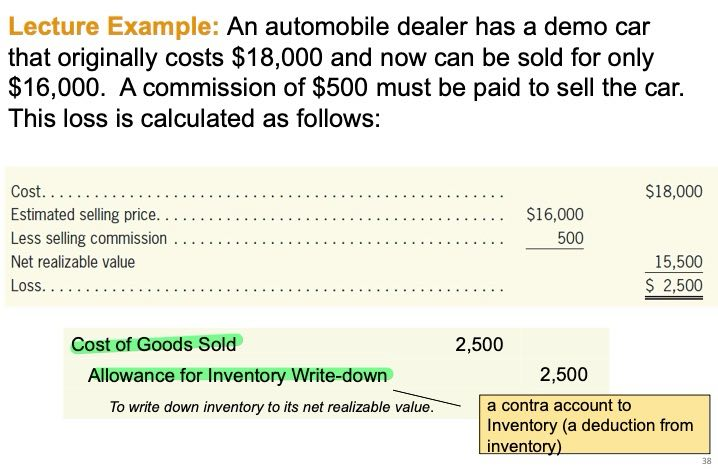
\includegraphics[width=0.9\linewidth]{NRV write-down.jpg}

  \section{Inventory Shrinkage}
  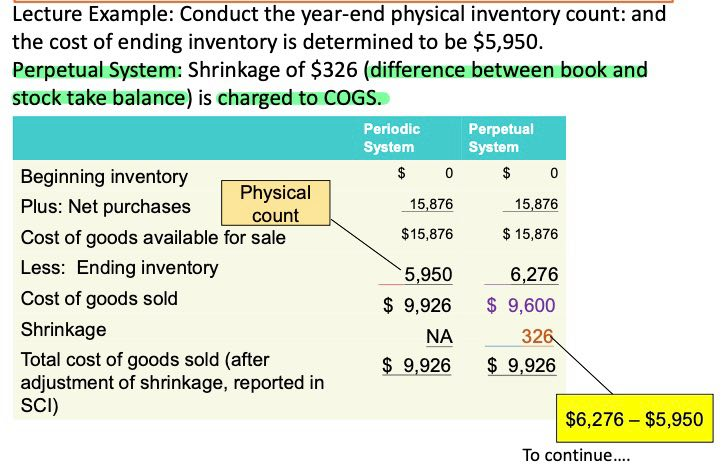
\includegraphics[width=0.8\linewidth]{Inventory shrinkage-1.jpg}
  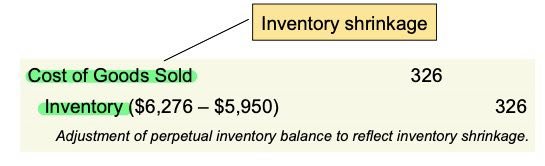
\includegraphics[width=0.8\linewidth]{Inventory shrinkage-2.jpg}

  \section{Net Purchase calc. under Periodic System}
  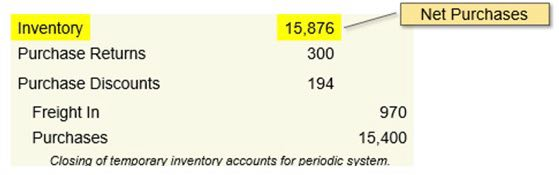
\includegraphics[width=1.0\linewidth]{Net Purchase calculation under Periodic System.jpg}

  \section{Statement of Comprehensive Income}
  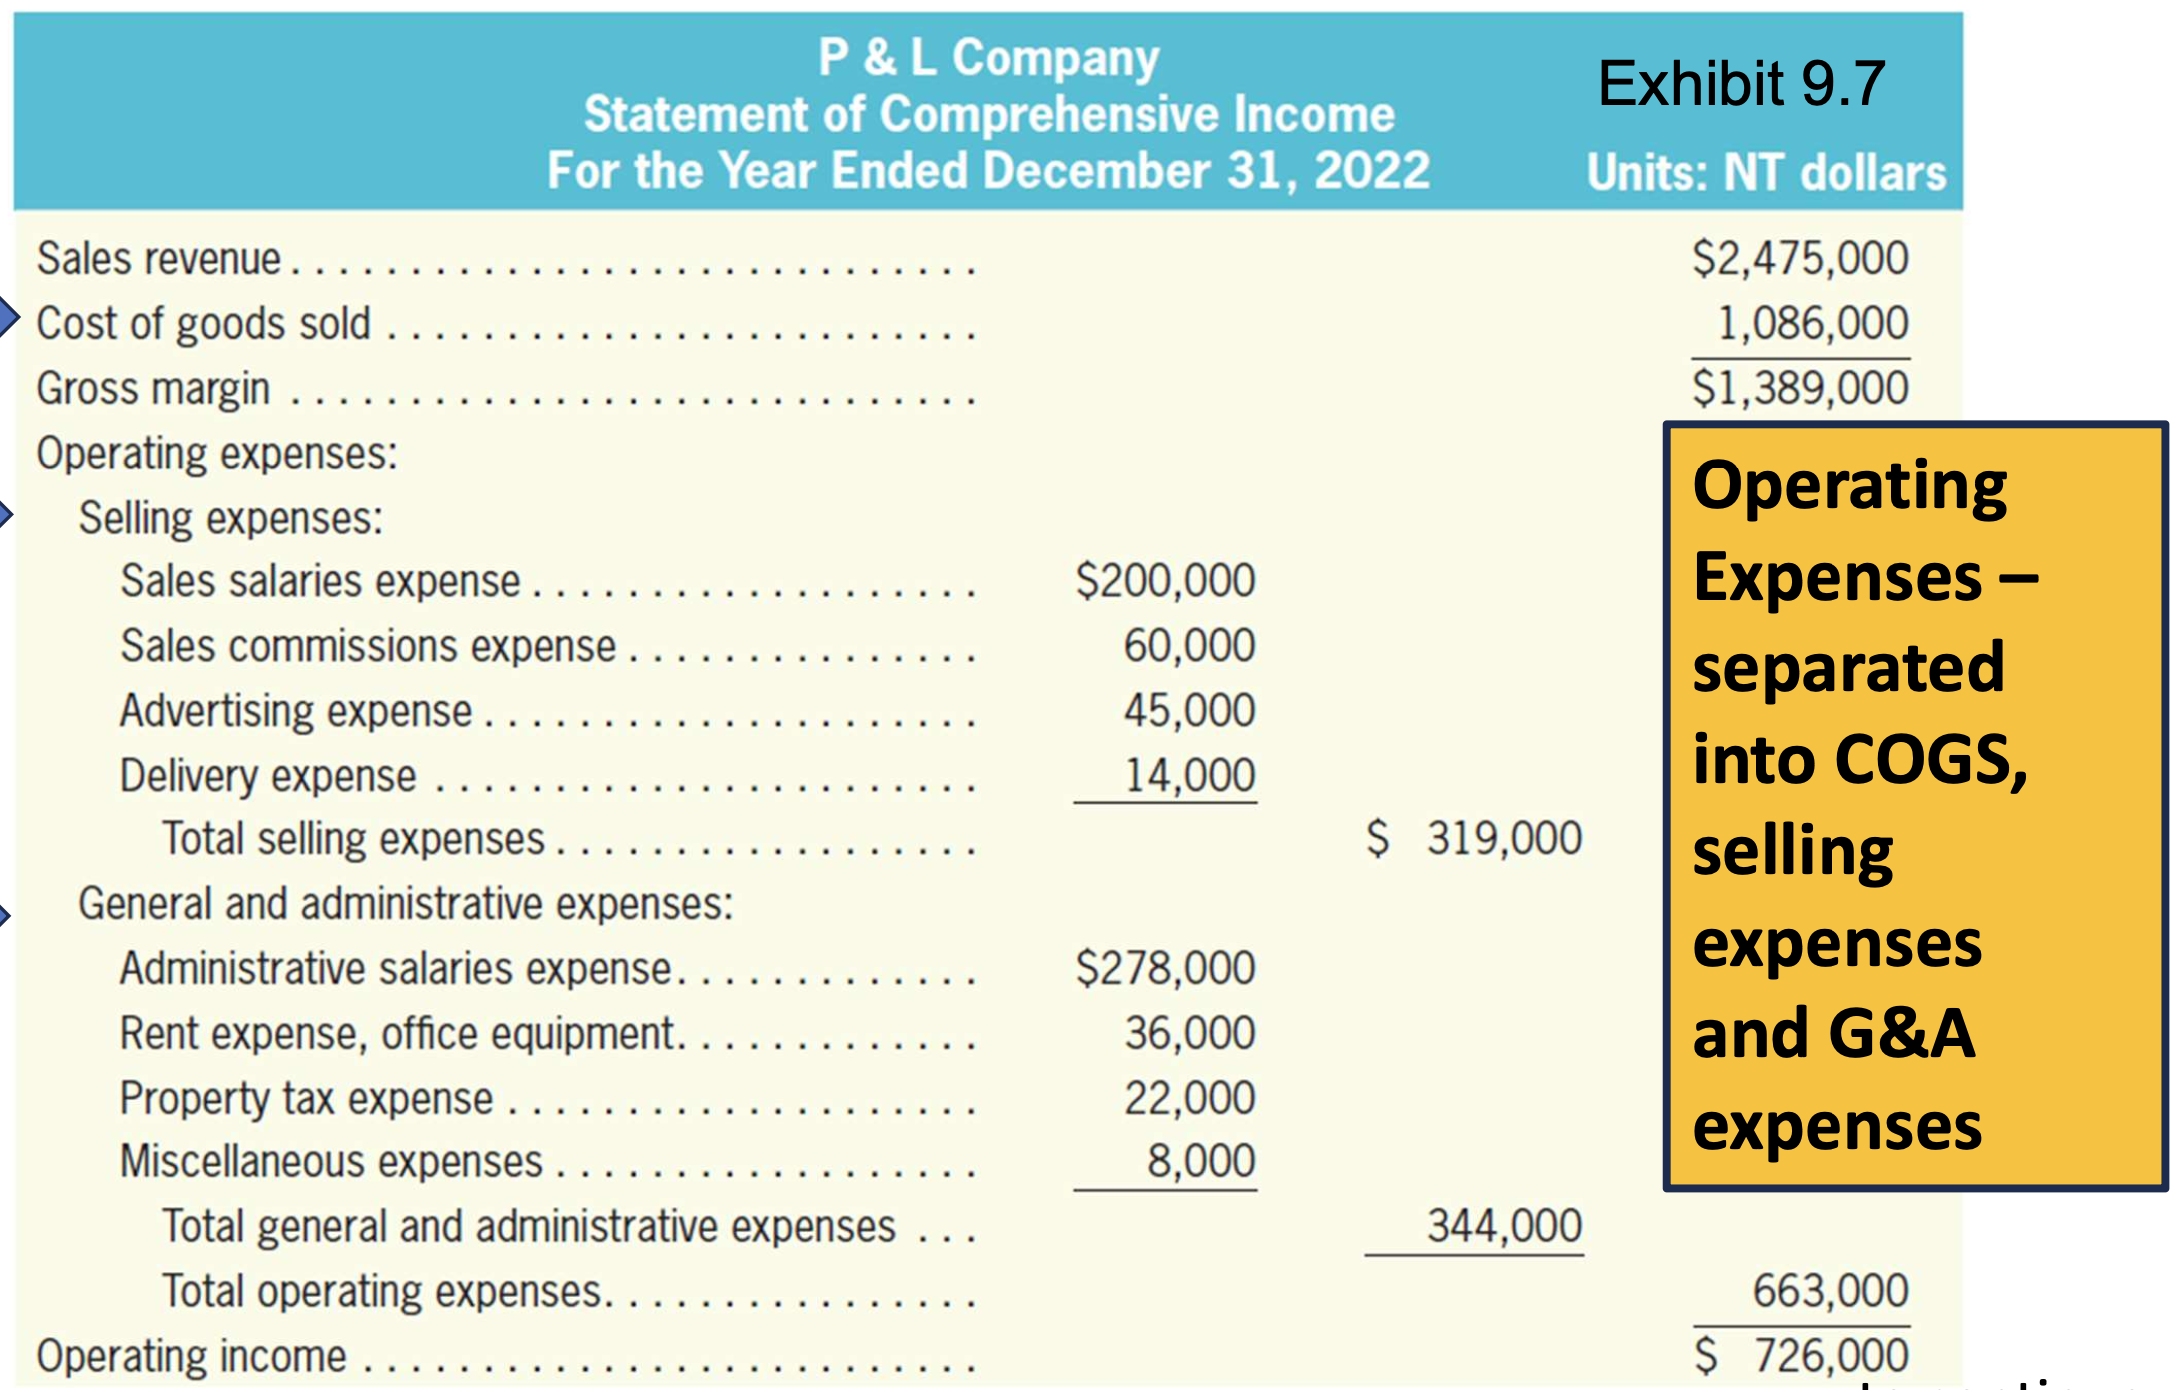
\includegraphics[width=1.0\linewidth]{SCI_updated_1.png} \\
  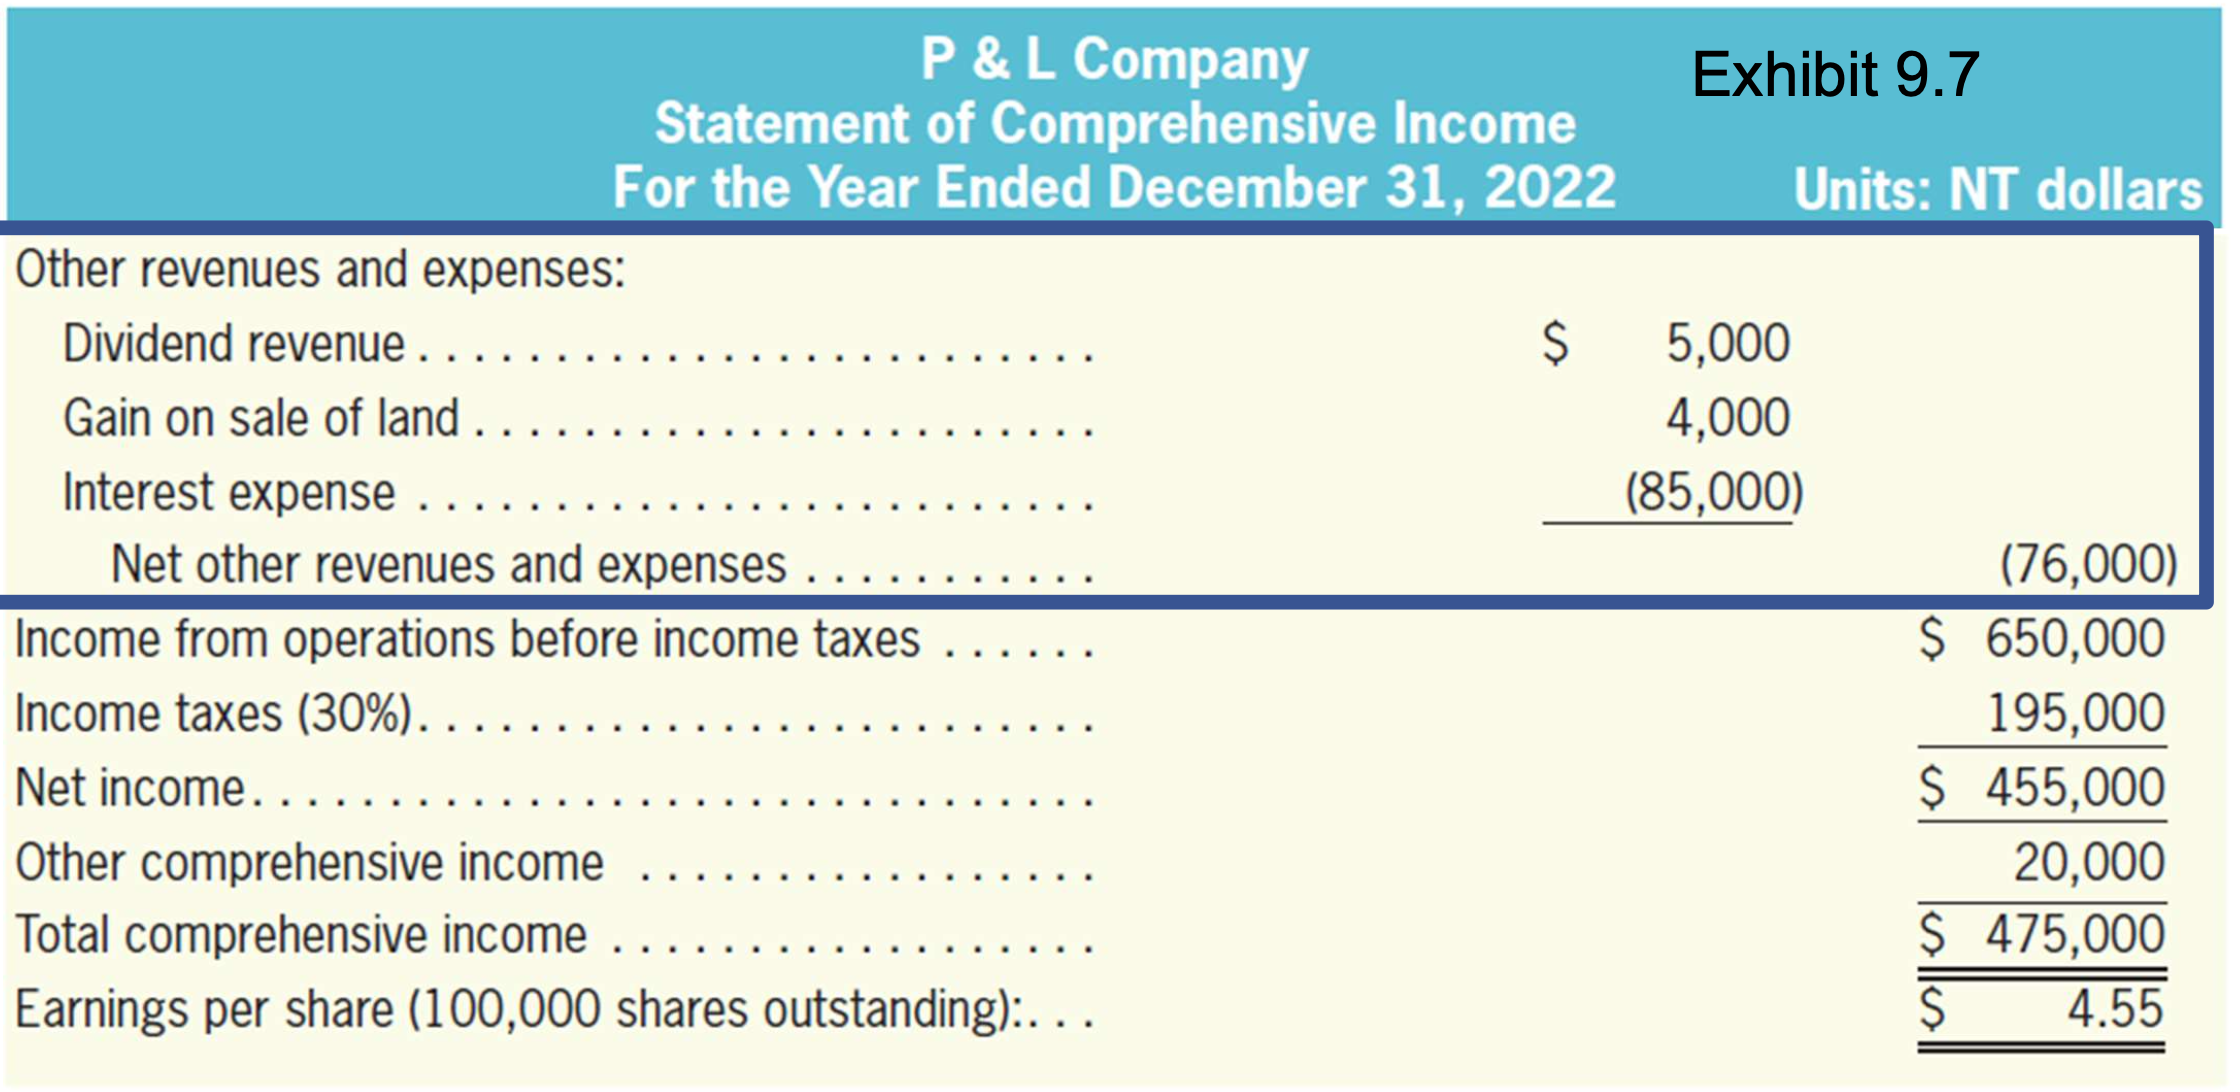
\includegraphics[width=1.0\linewidth]{SCI_updated_2.png}
\end{multicols*}
\end{document}
